During our research we also studied $GF(2^m)$ arithmetic for CPUs, where the coefficient bits are grouped into words. Most of the results were about polynomial reduction modulo a trinomial, a common operation in $\F_2[x]/(x^m+x^a+1)$. This type of field is interesting because it maximizes the number of zero coefficients in the the irreducible polynomial, enabling numerous simplifications. In turn, the reduction operation is used in multiplications and exponentiations, making speedups desirable.

Performing this operation in a CPU has a few differences from implementing a hardware circuit. For example, circuits often avoid irreducible polynomials with $a > m/2$. This is caused by the number of reduction steps in the standard technique, whcih represents inter-dependency of the calculations, and thus increases the maximum delay in a circuit. The maximum number $k$ of reduction steps for a trinomial 
$x^{m} + x^{a} + 1$ in terms of the exponent 
$a$ is given by Sunar and Ko\c{c} \cite{sunar1999mastrovito}
\begin{equation} \label{eq:k}
  k = \left \lfloor \frac{m-2}{m-a} \right \rfloor + 1.
\end{equation}

However, the number of reduction steps does not affect software implementations. To illustrate this, we take two algorithms that perform modular reduction for the NIST polynomials $x^{233} + x^{74} + 1$ and $x^{409} + x^{87} + 1$~\cite[p. 55]{hankerson2006guide}. Then we manually adapt each of these algorithms to perform a reduction modulo its reciprocal $x^m + x^{a-m} + 1$. Notice the only change required is in the indexing and bitwise shifts. The total number of operations remains the same. Algorithms meant for circuit implementations, on the other hand, would have different delay characteristics when 

To illustrate this, consider the following four CPU-targeted reduction algorithms: $x^{233} + x^{74} + 1$ and $x^{409} + x^{87} + 1$~\cite[p. 55]{hankerson2006guide}, and our adaptations. The second algorithm is our adaption to perform a polynomial reduction modulus $x^{233} + x^{159} + 1$, its reciprocal. Notice they perform exactly the same number of operations, but would have drastically different performance if implemented in hardware.


\begin{algorithm}
\begin{algorithmic}[1]
  \REQUIRE $C[2m-2,0]$
  \ENSURE $C[m-1,0]$
  \FOR{$i \gets 15$ \textbf{downto} $8$}
    \STATE $T \gets C[i]$
    \STATE $C[i-8] \gets C[i-8] \oplus T << 23$
    \STATE $C[i-7] \gets C[i-7] \oplus T >> 9$
    \STATE $C[i-5] \gets C[i-5] \oplus T << 1$
    \STATE $C[i-4] \gets C[i-4] \oplus T >> 31$
  \ENDFOR
  \STATE $T \gets C[7] >> 9$
  \STATE $C[0] \gets C[0] \oplus T$
  \STATE $C[2] \gets C[2] \oplus T << 10$
  \STATE $C[3] \gets C[3] \oplus T >> 22$
  \STATE $C[7] \gets C[7] \& \texttt{0x1FF}$
  \RETURN $C$
  \caption{Hankerson's algorithm for reduction modulus $x^{233} + x^{74} + 1$, a standardized NIST polynomial.}
  \label{alg:233_74_nist}
\end{algorithmic}
\end{algorithm}

 \begin{algorithm}
 \begin{algorithmic}[1]
  \REQUIRE $C[2m-2,0]$
  \ENSURE $C[m-1,0]$
  \FOR{$i \gets 14$ \textbf{downto} $8$}
    \STATE $T \gets C[i]$
    \STATE $C[i-8] \gets C[i-8] \oplus T << 23$
    \STATE $C[i-7] \gets C[i-7] \oplus T >> 9$
    \STATE $C[i-3] \gets C[i-3] \oplus T << 22$
    \STATE $C[i-2] \gets C[i-2] \oplus T >> 10$
  \ENDFOR
  \STATE $T \gets C[7] >> 9$
  \STATE $C[0] \gets C[0] \oplus T$
  \STATE $C[2] \gets C[2] \oplus T << 31$
  \STATE $C[3] \gets C[3] \oplus T >> 1$
  \STATE $C[7] \gets C[7] \& \texttt{0x1FF}$
  \RETURN $C$
  \caption{Algorithm for reduction modulus $x^{233} + x^{159} + 1$, $(233, 74)$'s recriprocal.}
  \label{alg:233_159}
\end{algorithmic}
\end{algorithm}

\begin{algorithm}
\begin{algorithmic}[1]
  \REQUIRE $C[2m-2,0]$
  \ENSURE $C[m-1,0]$
  \FOR{$i \gets 25$ \textbf{downto} $13$}
    \STATE $T \gets C[i]$
    \STATE $C[i-13] \gets C[i-13] \oplus T << 7$
    \STATE $C[i-12] \gets C[i-12] \oplus T >> 25$
    \STATE $C[i-11] \gets C[i-11] \oplus T << 30$
    \STATE $C[i-10] \gets C[i-10] \oplus T >> 2$
  \ENDFOR
  \STATE $T \gets C[12] >> 25$
  \STATE $C[0] \gets C[0] \oplus T$
  \STATE $C[2] \gets C[2] \oplus T << 23$
  \STATE $C[12] \gets C[12] \& \texttt{0x1FFFFFF}$
  \RETURN $C$
  \caption{Hankerson's algorithm for reduction modulus $x^{409} + x^{87} + 1$, a standardized NIST polynomial.}
  \label{alg:409_87_nist}
\end{algorithmic}
\end{algorithm}


\begin{algorithm}
\begin{algorithmic}[1]
  \REQUIRE $C[2m-2,0]$
  \ENSURE $C[m-1,0]$
  \FOR{$i \gets 25$ \textbf{downto} $13$}
    \STATE $T \gets C[i]$
    \STATE $C[i-13] \gets C[i-13] \oplus T << 7$
    \STATE $C[i-12] \gets C[i-12] \oplus T >> 25$
    \STATE $C[i-3] \gets C[i-3] \oplus T << 9$
    \STATE $C[i-2] \gets C[i-2] \oplus T >> 23$
  \ENDFOR
  \STATE $T \gets C[12] >> 25$
  \STATE $C[0] \gets C[0] \oplus T$
  \STATE $C[10] \gets C[10] \oplus T << 2$
  \STATE $C[12] \gets C[12] \& \texttt{0x1FFFFFF}$
  \RETURN $C$
  \caption{Algorithm for reduction modulus $x^{409} + x^{322} + 1$, $(409, 87)$'s reciprocal.}
  \label{alg:409_322}
\end{algorithmic}
\end{algorithm}

\section{Choice of $a$}

The choice of the second coefficient $a$ directly affects the performance characteristics of reduction algorithms. Several factors are at play:

\begin{itemize}
\item The number of reduction steps depends on the proximity of $a$ and $m$. The number of steps increases with $a$, in discrete steps.
\item The number of reduction steps affects the depth of the circuit when implemented in hardware, though usually in logarithm fashion.
\item If $m-a < W$ software implementations will be less efficient. This is because there will be XOR operations inside words, and the operations can not be performed with full word-sized XORs.
\item The alignment of $a$ and $m-a$ with relation to $W$ define if word-sized XORs will require bits of two words in the source or in the destination. Thus alignment can halve the number of operations involved.
\end{itemize}

\section{Existing algorithms}\label{existing-algorithms}

Masoleh \cite[p. 953]{Masoleh} presents a recursive multiplier algorithm with $N_\oplus = m^2-1$ for $x^m + x^a + 1$ and $N_\oplus = m^2-\frac{m}{2}$ if $a = \frac{m}{2}$. If we consider that the multiplication takes ${(m-1)}^2$ XORs, then, the number of XORs for the reduction is $2m-2$ and $\frac{3}{2}m-1$, respectively. 

{[}NIST, Scott, etc. just dry descriptions{]}

\section{Reduction equation}

[This is an attempt to formulate the reduction operation as an equation. This is useful for proving correctness of algorithms by showing equivalence to the equations. I'm not 100\ they are correct. (I think they are not truncating the value to the modulus degree, but that should be easy to fix)]

General polynomial reduction equation with coefficients in $GF(2)$, with reduction steps in evidence:

\begin{gather}
    \sum_{i = 0}^{2m - 2}{c_i x^i} \mod \sum_{i = 0}^{m}{k_i x^i} = \\
    \sum_{i = 0}^{m-1}{c_i x^i} + \sum_{i=0}^{\floor*{\frac{m - 2}{m - a}}}
        \sum_{l=0}^{m}{ \sum_{j = 0}^{m - 2 - ia}{k_l c_{j + m + ia} x^{j+l}}  }
\end{gather}

General trinomial reduction equation ($1 \le a < m$), with reduction steps in evidence:

\begin{gather}
    \sum_{i = 0}^{2m - 2}{c_i x^i} \mod x^m + x^a + 1 = \\
    \sum_{i = 0}^{m-1}{c_i x^i} + \sum_{i=0}^{\floor*{\frac{m - 2}{m - a}}} \left(
        \sum_{j = 0}^{m - 2 - ia}{c_{j + m + ia} x^j} +
        \sum_{j = 0}^{m - 2 - ia}{c_{j + m + ia} x^{j+a}}
    \right) 
\end{gather}

Special case $a=1$ (single step):

\begin{gather}
    \sum_{i = 0}^{m-1}{c_i x^i} +
        \sum_{j = 0}^{m - 2}{c_{j + m} x^j} +
        \sum_{j = 0}^{m - 2}{c_{j + m} x^{j+a}}
\end{gather}

Special case $1 < a < \frac{m}{2}$ (two steps):

\begin{gather}
    \sum_{i = 0}^{m-1}{c_i x^i} +
        \sum_{j = 0}^{m - 2}{c_{j + m} x^j} +
        \sum_{j = 0}^{m - 2}{c_{j + m} x^{j+a}} +
        \sum_{j = 0}^{m - 2 - a}{c_{j + m + a} x^j} +
        \sum_{j = 0}^{m - 2 - a}{c_{j + m + a} x^{j+a}}
\end{gather}

Special case $a = \frac{m}{2}$ (two steps with cancellation):

\begin{gather}
    \sum_{i = 0}^{m-1}{c_i x^i} +
        \sum_{j = 0}^{\frac{m}{2} - 2}{c_{j + m} x^j} +
        \sum_{j = 0}^{m - 2}{c_{j + m} x^{j+\frac{m}{2}}} +
        \sum_{j = 0}^{\frac{m}{2} - 2}{c_{j + m + a} x^j}
\end{gather}


\section{Operating on words}\label{operating-on-words}

Bit manipulation operations are not efficiently supported in most programming languages. Programming languages, in general, are word oriented following a specific microprocessor architecture. For instance, numbers with $32$- or $64$-bit word size. The reduction algorithms themselves are strongly bit oriented. The codification of these algorithms to word oriented programming languages usually add some complexity in terms of new operations. Specific techniques that help us in this coding have been proposed in the literature\cite{Hilewitz2008}. 

Interoperability often means an irreducible polynomial must behave well
in both hardware and software implementations. A straightforward
approach to this problem is to develop a hardware implementation first,
XOR'ing individual bits, and convert the algorithm to words. This can be
thought of as parallelizing the operations, with SHIFTs and AND/OR masks
for alignment. This is the approach used in this document. {[}more
formalization? references of other similar approaches?{]}

The difficulty of the conversion process greatly varies depending on the
access pattern of the algorithm and alignment of words. If all coefficients inside a range are
XOR'ed once in a linear fashion, the XOR distance a multiple of the word size, and the start and end range lie in word boundaries, the converted algorithm gains a full
speedup of up to \texttt{WORD\_SIZE} times
{[}$C_{word} = \ceil*{\frac{C_{bit}}{W}}${]}.

\section{Bit operation reduction algorithms}\label{sec:bit:operation}
This section presents bit operation reduction algorithms for trinomials. The algorithms depend on the number of reduction steps given by Eq.~\ref{eq:k}. As $k$ increases, more steps can be required to perform the reduction. The equation $x^{m+j} \equiv x^{a+j} + x^j mod (x^m+x^a+1)$ is used to replace each coefficient at or over $m$ with a smaller one, reducing the polynomial. The Algorithm \ref{alg:bits} shows this reduction process. 

\begin{algorithm}
\begin{algorithmic}[1]
  \REQUIRE $a$, $C[2m-2,0]$
  \ENSURE $C[m-1,0]$
  \STATE $k \gets \left \lfloor \frac{m-2}{m-a} \right \rfloor + 1$
  \STATE $r \gets 0$
  \FOR{$i \gets 1$ \textbf{to} $k$}
    \STATE $r \gets r + (m-a)$
    \FOR{$j \gets 0$ \textbf{to} $m-1-r$}
      \STATE $C[j] \gets C[j] \oplus C[j+a+r]$
      \ENDFOR
    \FOR{$j \gets a$ \textbf{to} $m-1$}
      \STATE $C[j] \gets C[j] \oplus C[j+r]$
      \ENDFOR
    \ENDFOR
  \RETURN $C$
  \caption{General reduction algorithm processed by bit, taken directly from equation 5 (update).}
  \label{alg:bits}
\end{algorithmic}
\end{algorithm}

However this algorithm introduces a number of repeated bit operations. Some of these operations could be canceled, and others could be grouped, so that they can be made once and reused when necessary.

We propose a general algorithm for all possible values of $a$, and one for the special case $m=2a$. This is known in literature as Equally Spaced Polynomials. For comparison reasons we introduce instantiated algorithms for $a = 1$ and $a = m-1$, which are usually treated as special cases in the literature.

\subsection{Case $(m-a) \mid a$}

Situations where $m-a$ divides $a$ result in cancelled items, coefficients that are XORed twice to the same bit. The most visible case is when $m-a = a$, the equally-spaced trinomial. In this case, the cancelled items translate directly to cancelled operations, and the reduction can be performed in less steps.

Other cases can be found by using the formula $a = \frac{\alpha}{\alpha + 1}m$ with $a, \alpha \in \mathbb{Z}^{+}$ [I think it should be $\mathbb{N}$, Custodio disagrees]. The equally spaced case happens when $\alpha = 1$. As an example of other cases, $x^{20}+x^{15}+1$, $x^{20}+x^{16}+1$ and $x^{20}+x^{18}+1$ all contain some cancellations. The number of XOR cancellations is $m - a - 1$, which explains the complexity of $\frac{3}{2}m - 3$ for the equally-spaced case. It's still an open problem if the non-equally spaced case can be optimized at all.

\subsection{Case $a=1$}
When $a=1$, the number of reduction steps given by the Eq.~\ref{eq:k} is $$k=\left \lfloor \frac{m-2}{m-a} \right \rfloor + 1=\left \lfloor \frac{m-2}{m-1} \right \rfloor + 1=1.$$ This is the simplest case. The number of XOR operations is $N_\oplus = 2m-2$.

 \begin{algorithm}
 \begin{algorithmic}[1]
  \REQUIRE $m$, $C[2m-2,0]$
  \ENSURE $C[m-1,0]$
  \FOR{$i \gets m-2$ \textbf{downto} $0$}
      \STATE $C[i+1] \gets C[i+1] \oplus C[i+m]$
      \STATE $C[i] \gets C[i] \oplus C[i+m]$
  \ENDFOR
  \RETURN $C$
  \caption{Simple reduction algorithm for $x^m + x + 1$, $a = 1$}
  \label{alg:a1:bit:operation}
\end{algorithmic}
\end{algorithm}

Algorithm \ref{alg:a1:bit:operation}  uses $2m - 2$ operations and has a depth of only 2. This is the best possible case for a bit-parallel circuit.

\subsection{Case $ 1 < a < \frac{m}{2}$}
The number of reduction steps given by the Eq.~\ref{eq:k} is $$k=\left \lfloor \frac{m-2}{m-a} \right \rfloor + 1=2.$$ The number of XOR operations is $N_\oplus = 2m-2$.

\subsection{Case $m=2a$}
The special case where $m=2a$ operation algorithm is presented in Algorithm~\ref{alg:esp}. This algorithm, known in literature as Equally Spaced Trinomial, is essentially the same stated by Wu\cite[p. 753, Eq. 3]{Wu2002}. There, however, it used different vectors: one for the element to be reduced and other for the result itself. The number of reduction steps given by the Eq.~\ref{eq:k} is $$k=\left \lfloor \frac{m-2}{m-a} \right \rfloor + 1=\left \lfloor \frac{2a-2}{2a-a} \right \rfloor + 1=\left \lfloor \frac{2a-2}{a} \right \rfloor + 1=2.$$ 

\ref{alg:equallyspaced:bit:operation} is a $m=2a$ version of algorithm \ref{alg:general:bit:operation} with cancellations. It is trivial to see that its complexity is $m + a - 1$, or, since $a = m/2$, the number of operations is exactly $\frac{3}{2}m - 1$.

\begin{algorithm}
\begin{algorithmic}[1]
  \REQUIRE $a$, $C[0,2m-2]$
  \ENSURE $C[m-1,0]$
  \FOR{$i \gets 0$ \textbf{to} $m-2$}
    \STATE $C[i+a] \gets C[i+a] \oplus C[i+m]$
    \ENDFOR
  \FOR{$i \gets a - 1$ \textbf{to} $0$}
    \STATE $C[i] \gets C[i] \oplus C[i+m]$
    \ENDFOR
  \RETURN $C$
  \caption{Simple Reduction algorithm for $x^{m} + x^a +1$, $a = \frac{m}{2}$.}
  \label{alg:equallyspaced:bit:operation}
\end{algorithmic}
\end{algorithm}

\subsubsection{Proof}

Applying the equation of maximum number of reduction steps, by Sunar and Ko\c{c} \cite{SunarKoc}, to the equally spaced case we arrive at

\begin{equation}
  k = \left \lfloor \frac{m-2}{m-\frac{m}{2}} \right \rfloor + 1 = 2
\end{equation}

Therefore the reduction equation is comprised of two steps. Since $(x^m)^n = (x^a + 1)^n$, the full reduction formula for the equally spaced trinomial is:

\begin{gather}
    \sum_{i = 0}^{m-1}{c_i x^i} +
        \sum_{j = 0}^{\frac{m}{2} - 2}{c_{j + m} x^j} +
        \sum_{j = 0}^{m - 2}{c_{j + m} x^{j+\frac{m}{2}}} +
        \sum_{j = 0}^{\frac{m}{2} - 2}{c_{j + m + a} x^j}
\end{gather}

Lines 1 and 2 of algorithm \ref{alg:equallyspaced:bit:operation} correspond to the first reduction step for $x^a$ (last summation). Lines 3 and 4 correspond truncated first step for $x^0$ (second summation). And because of the mutable nature of the data structure, lines 3 and 4 operate on bits that were already XOR'ed in the first loop. This overlap gives raises to the remaining $a$ elements of the second reduction step for $x^0$ (third summation).

End of proof.

\begin{algorithm}
\begin{algorithmic}[1]
  \REQUIRE $a$, $C[4a-2,0]$
  \ENSURE $C[2a-1,0]$
  \FOR{$i \gets 0$ \textbf{to} $a-2$}
    \STATE $C[i] \gets C[i] \oplus C[i+2a] \oplus C[i+3a]$
    \ENDFOR
  \STATE $C[a-1] \gets C[a-1] \oplus C[3a-1]$ 
  \FOR{$i \gets a$ \textbf{to} $2a-1$}
    \STATE $C[i] \gets C[i] \oplus C[i+a]$
  \ENDFOR
  \RETURN $C$
  \caption{Reduction algorithm for $x^{m} + x^a +1$, $m=2a$.}
  \label{alg:esp}
\end{algorithmic}
\end{algorithm}

\subsection{Case $a=m-1$}
The special case where $a=m-1$ operation algorithm is presented in Algorithm~\ref{alg:ma1}. This algorithm has the same complexity as the general algorithm, i.e, $N_\oplus = 2m-2$. The number of reduction steps given by the Eq.~\ref{eq:k} is $$k=\left \lfloor \frac{m-2}{m-a} \right \rfloor + 1 = \left \lfloor \frac{m-2}{m-(m-1)} \right \rfloor + 1 = \left \lfloor m-2 \right \rfloor + 1=m-1.$$

\begin{algorithm}
\begin{algorithmic}[1]
  \REQUIRE $a$, $C[2m-2,0]$
  \ENSURE $C[m-1,0]$
  \FOR{$i \gets 2m-3$ \textbf{downto} $m$}
    \STATE $C[i] \gets C[i] \oplus C[i+1]$
    \ENDFOR
  \STATE $C[a] \gets C[a] \oplus C[m]$ 
  \FOR{$i \gets 0$ \textbf{to} $m-2$}
    \STATE $C[i] \gets C[i] \oplus C[i+m]$
  \ENDFOR
  \RETURN $C$
  \caption{Reduction algorithm for $x^{m} + x^a +1$, $a=m-1$.}
  \label{alg:ma1}
\end{algorithmic}
\end{algorithm}

\subsection{First General case for $1 \leq a < m$}
The general bit operation algorithm is presented in Algorithm~\ref{alg:general:bit:operation}.

\begin{algorithm}
\begin{algorithmic}[1]
  \REQUIRE $m$, $a$, $C[2m-2,0]$
  \ENSURE $C[m-1,0]$
  \FOR{$i \gets m-2$ \textbf{downto} $0$}
      \STATE $C[i+a] \gets C[i+a] \oplus C[i+m]$
      \STATE $C[i] \gets C[i] \oplus C[i+m]$
  \ENDFOR
  \RETURN $C$
  \caption{Simple reduction algorithm for $x^m + x^a +1$, $m \not = 2a$}
  \label{alg:general:bit:operation}
\end{algorithmic}
\end{algorithm}

This algorithm obviously uses $2 (m - 1) = 2m -2$ XORs.

\section{Word operation reduction algorithms}

\subsection{Notations}
In this paper, we assume that one word has $W$ bits where $W$ is a multiple of $8$. The bits of a word $A$ are numbered from $0$ to $W-1$, with the rightmost bit (LSB) of $A$ designated as bit $0$. The following standard notation is used to denote operations on words $A$ and $B$:\\

\begin{tabular}{ll}
  $A \BitXOR B$ & bitwise exclusive or. \\
  $A \BitOr B$ & bitwise or. \\
  $A \BitAnd B$     & bitwise $AND$. \\ 
  $A \ShiftLeft n$     & left shift of $A$ by $n$ positions, ($n<W$), with the bits from 0 to $n-1$ set to $0$. \\
  $A\ShiftRight n$    & righ shift of $A$ by $n$ positions, ($n<W$), with bits from $W-n$ to $W-1$ set to $0$. \\
  $C$ & Vector os bits.\\
  $D$ & Array de elements of $W$ bits. \\
  $D_{Red}$ & Reduced element. \\
\end{tabular}\\

Figure~\ref{fig:elemento:field} shows the representation of a element $d \in \ftwom$ as an array $D$ of $t$ words of $W$ bits, where $t = \left \lceil \frac{m}{W} \right \rceil$. The $s = tW-m$ highest order bits of $D[t-1]$ are not unused.
\begin{figure}[htb]
  \centering
  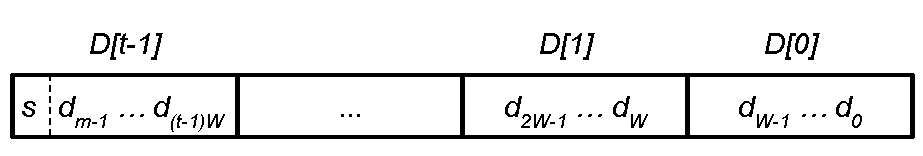
\includegraphics[width = .55\columnwidth]{figures/element-word.pdf}
\caption{Representation of $d \in \ftwom$ as an array $D$ of $W$ bit words. The $s = tW-m$ highest order bits of $D[t-1]$ are not unused.}
\label{fig:elemento:field}
\end{figure}
\\

For the case where $(m-1) \mod{W} > \frac{W}{2}$, the Figure~\ref{fig:elemento:field:mult} shows the representation of a element $d = ab$, $a,b \in \ftwom$ as an array $D$ of $W$-bit words. The $s = 2(tW-m)+1$ highest order bits of $D[2t-1]$ are not unused.

\begin{figure}[htb]
  \centering
  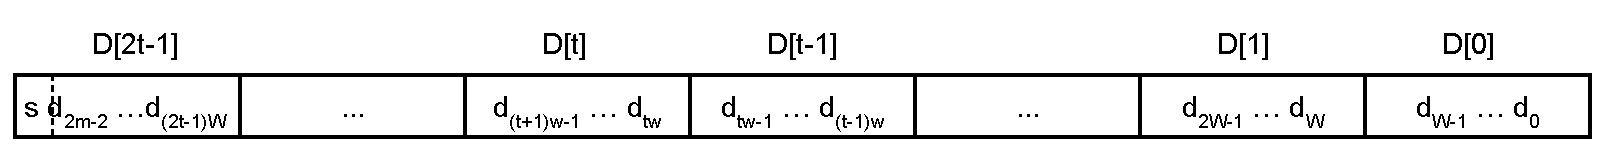
\includegraphics[width = .9\columnwidth]{figures/two-word-element-1.pdf}
\caption{Representation of $d = ab$, $a,b \in \ftwom$ as an array $D$ of $W$-bit words. The $s = 2(tW-m)+1$ highest order bits of $D[2t-1]$ are not unused.}
\label{fig:elemento:field:mult}
\end{figure}


When $(m-1) \mod{W} \leq \frac{W}{2}$, $D[2t-1]$ is not needed.  Figure~\ref{fig:elemento:field:mult2} shows the representation of a element $d = ab$, $a,b \in \ftwom$ as an array $D$ of $W$-bit words. The $s = 2(tW-m)+1$ highest order bits of $D[2t-2]$ and $D[2t-1]$ are not unused.
\begin{figure}[htb]
  \centering
  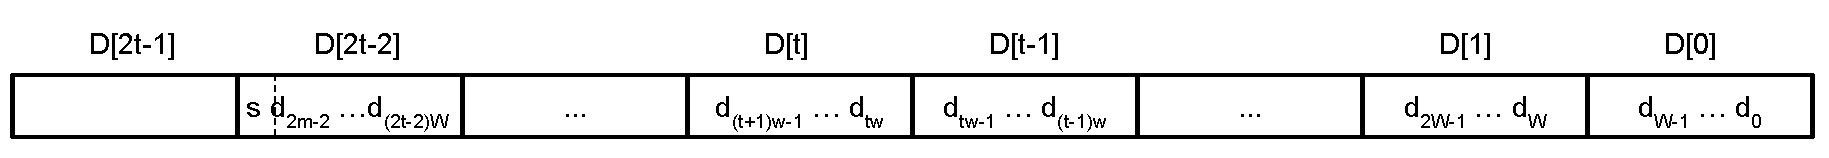
\includegraphics[width = \columnwidth]{figures/two-word-element-2.pdf}
\caption{Representation of $d = ab$, $a,b \in \ftwom$ as an array $D$ of $W$-bit words. The $s = 2(tW-m)+1$ highest order bits of $D[2t-2]$ and $D[2t-1]$ are not unused.}
\label{fig:elemento:field:mult2}
\end{figure}

In these cases a whole word is wasted, but length calculations become simpler: to get the length (in words) of a product of two elements, just add their lengths (in words).

\subsection{Algorithms}
The processing algorithms by word found in the literature for the irreducible polynomials are an implementation using words of the general algorithm~\ref{alg:bits} of bits. These algorithms, therefore, do not take into account the possible redundant operations inside. One explanation for this could be the fact that for the small middle exponents, this redundancy is small, almost negligible. However, for large exponents the redundancy increases considerably. If the algorithm benefit from these redundancies, you can get algorithms as effective as, or perhaps even better, for irreducibles with great exponents. \\

{\bf Custodio} Teremos nessa seção: \\
a) Reducao por bit usando palavras\\
b) Redução usando palavras do algoritmo geral de bits;\\
c) Algoritmos do NITS por palavra;\\
d) Nossos algoritmos otimizados ( $a=m/2$, $a \neq m/2$ ) processados por palavras;\\
e) Novos algoritmos para os trinomios do NITS mas usando feito usando nosso algoritmo otimizado para a primeira faixa de $a$;\\
 

\subsection{General by word bit processing}
For low weight irreducible polynomials with middle terms close to each other or, in particular, trinomials, the reduction may be performed efficiently by words as shown in Algorithm~\ref{alg:wordbit:hankerson}\cite[p. 53]{Hankerson}. In this algorithm $$r(x) = f(x) + x^m$$\\

{\bf Custodio} Verificar o algorithm. Explicar ( modificar ) $C\{j\}$. Fazer uma figura semelhante a Fig. 2.9 do Hankerson para explicar de forma geral este algoritmo. Apresentar uma análise de complexidade para este algoritmo. Por exemplo, a soma re $u_k$ pode ser feita por um $for$ de $W$ passos.

\begin{algorithm}
\begin{algorithmic}[1]
  \REQUIRE $C[2m-2,0]$, $W$
  \ENSURE $C[m-1,0]$
  {\it Precomputation}. Compute $u_k = x^k r(x)$, $0 \leq k \leq W-1$ 
  \FOR{$i \gets 2m-2$ \textbf{downto} $m$}
    \IF{$C[i]=1$}
      \STATE $j \gets \left \lfloor \frac{i-m}{W} \right \rfloor$
      \STATE $k \gets (i-m) - Wj$
      Add $u_k(x)$ to $C\{j\}$
    \ENDIF
  \ENDFOR
  \RETURN $C$
  \caption{Reduction algorithm by word (one bit at a time) (Hankerson).}
  \label{alg:wordbit:hankerson}
\end{algorithmic}
\end{algorithm}

\subsection{Word operation of the case $a=1$}\label{sec:word:operation:alg:a1}
Figure \ref{fig:word:operation:alg:a1} is a representation of the case $a=1$ and $(m-1) \mod{W} > \frac{W}{2}$. In the figure, $D$ is the element to be reduced, $D_a$ are the bits reduced by the exponent $a$ and $D_0$ are the bits reduced by $0$. $D_{Red} = D \BitXOR D_a \BitXOR D_0$ is the reduced element. The hatched bits (shaded in figure) should be set to 0.
\begin{figure}[htb]
  \centering
  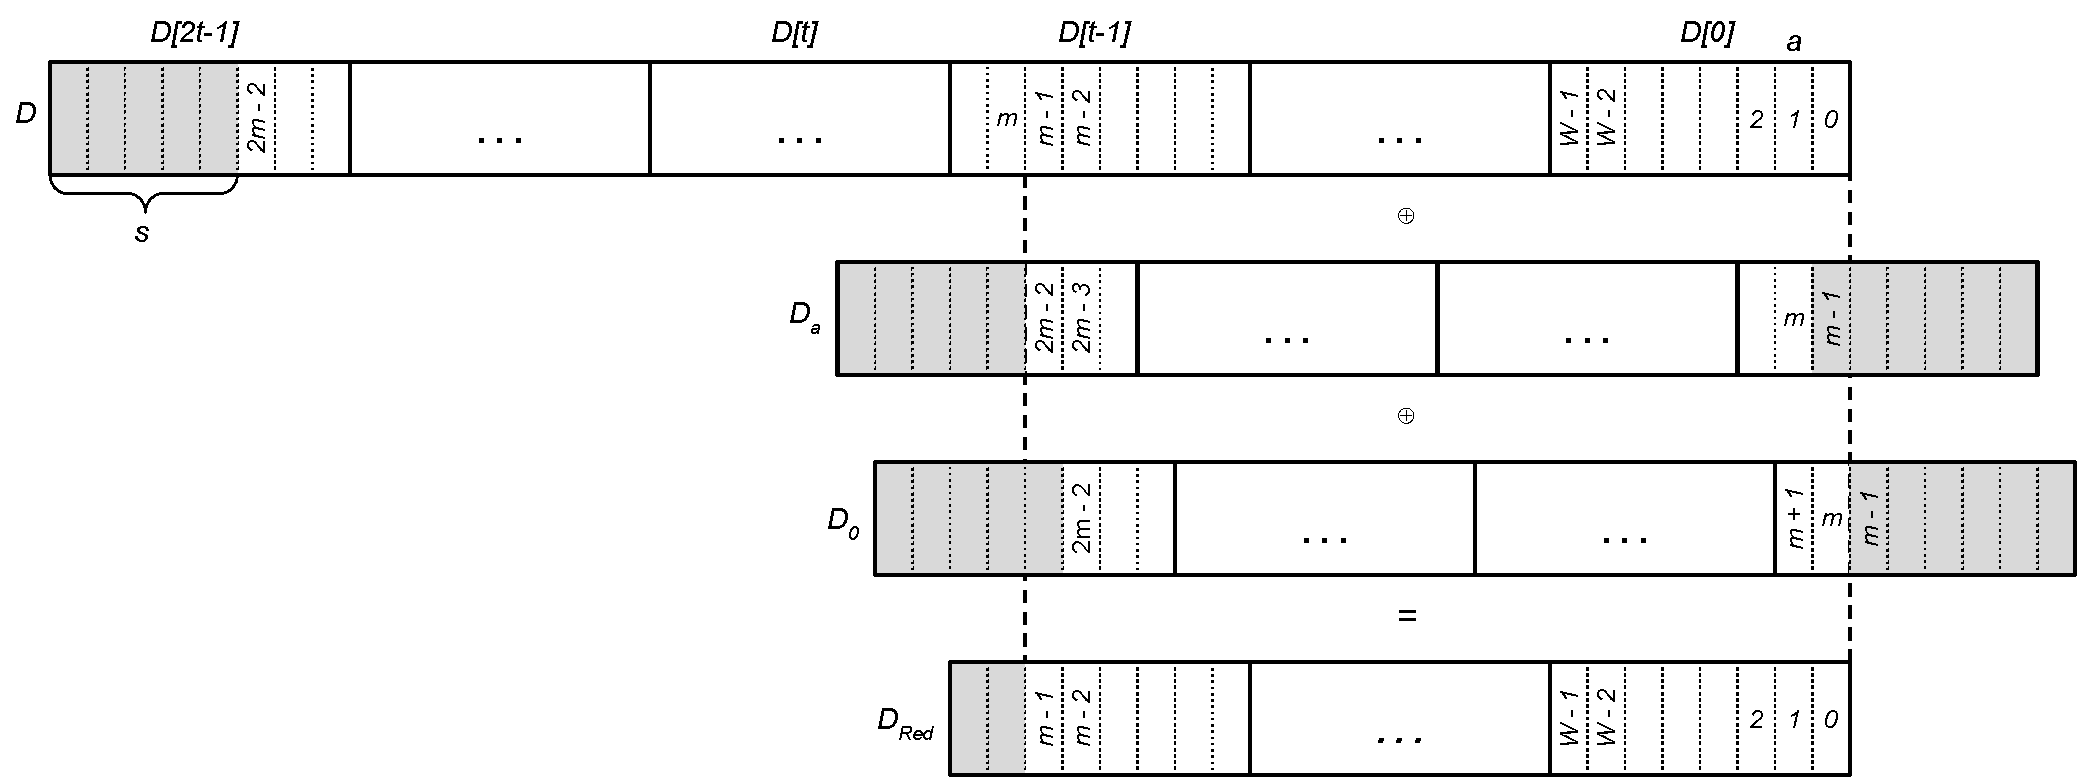
\includegraphics[width = \columnwidth]{figures/two-elements-reduction-a-1.pdf}
\caption{Word operation of the case $a=1$.}
\label{fig:word:operation:alg:a1}
\end{figure}
\\

\begin{algorithm}
  \begin{algorithmic}[1]
  \REQUIRE $D[2t-1,0]$,$t$, $m$, $W$
  \ENSURE $D_{Red = D[t-1,0]}$
  \STATE $u \gets tW - m$
  \STATE $h \gets W - u$
  \STATE $T \gets D[t-1] \ShiftRight h$
  \STATE $D[0] \gets D[0] \oplus T \oplus (D[t] \ShiftLeft u) \oplus (T \ShiftLeft 1) \oplus (D[t] \ShiftLeft (u+1)$ \label{alg:a1:high:primeira-linha}
  \FOR{$i \gets 1$ \textbf{to} $t-2$}
    \STATE $D[i] \gets D[i] \oplus (D[i+t-1] \ShiftRight h) \oplus (D[i+t-1] \ShiftRight (h-1)) \oplus (D[i+t] \ShiftLeft u) \oplus (D[i+t] \ShiftLeft (u+1))$
    \ENDFOR
  \STATE $T \gets D[2t-1] \ShiftLeft (2u+1)$\ \COMMENT{This avoid using \& to reset unused bits}
  \STATE $D[t-1] \gets D[t-1] \oplus (D[2t-2] \ShiftRight h) \oplus (D[2t-2] \ShiftRight (h-1)) \oplus (T \ShiftRight u) \oplus (T \ShiftRight (u+1))$
  \RETURN $D_{Red}$
  \caption{Reduction algorithm by word for $x^m + x + 1$, from $D[2t-1]$.}
  \label{alg:word:a1:high}
\end{algorithmic}
\end{algorithm}

We have $4$ XORs in line \ref{alg:a1:high:primeira-linha}, $4(t-2)$ XORs in line 5, and $4$ XORs in line 8. The total is $$N_\oplus = 4t.$$

We have $$N_{Shifts} = 4t.$$

Now, we have the case where $(m-1) \mod{W} \leq \frac{W}{2}$. In this case, $D[2t-2]$ is not used as show in Figure \ref{fig:word:operation:alg:a1:low}. Thus, the algorithm procede to reduce the bits from $D[2t-1]$. The Algorithm is show in \ref{alg:word:a1:low}.

\begin{figure}[htb]
  \centering
  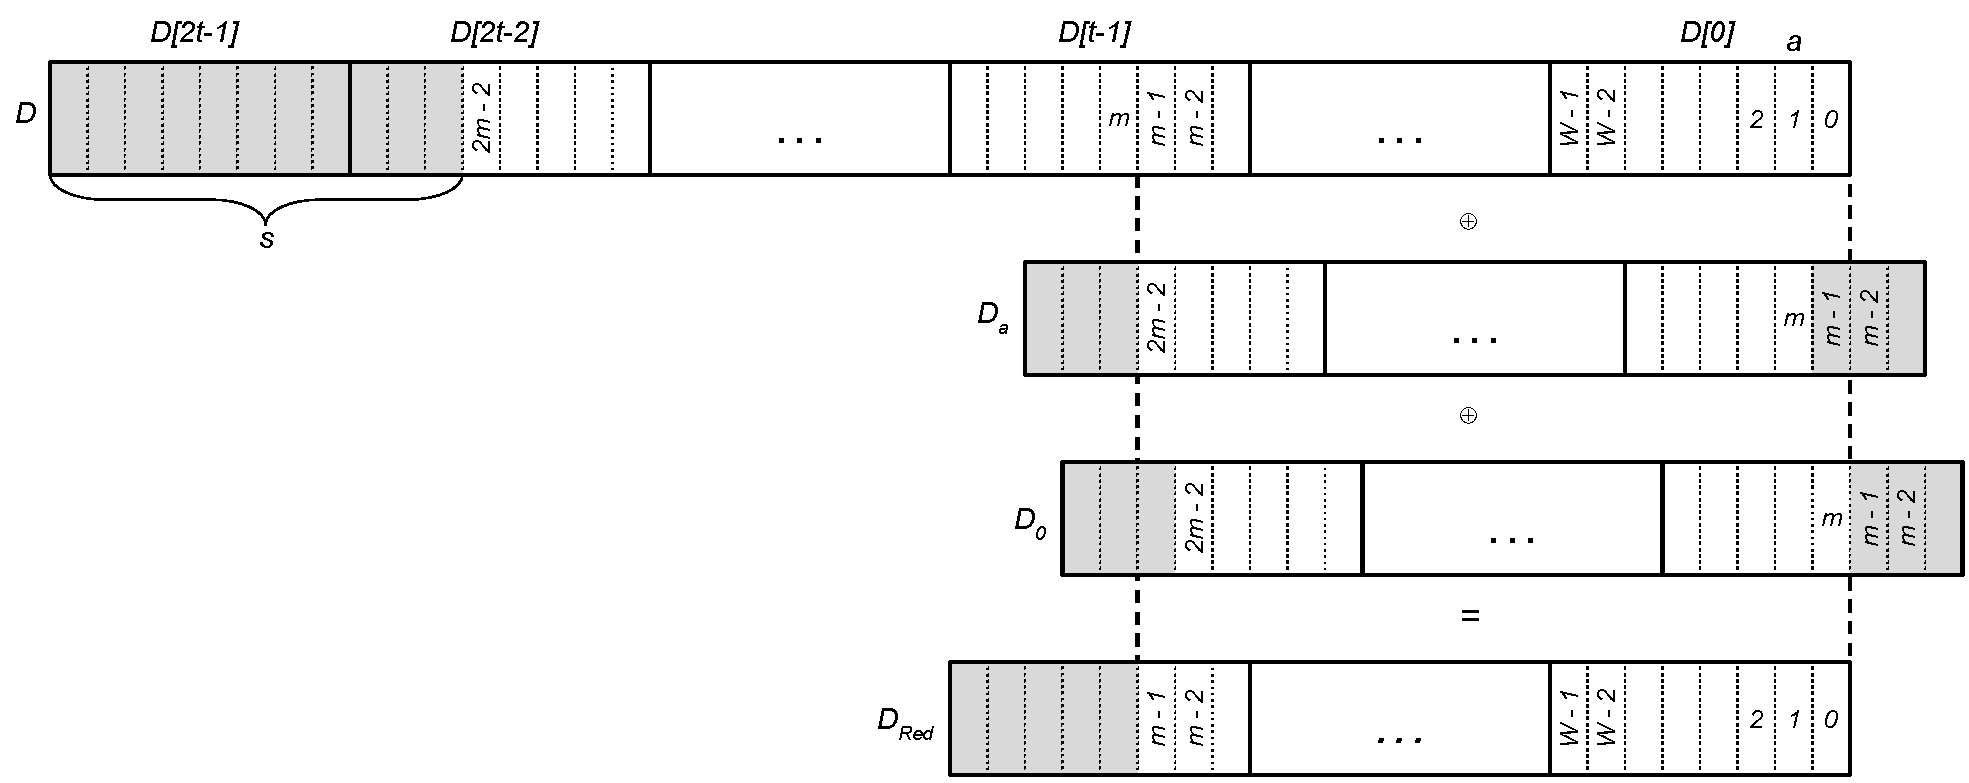
\includegraphics[width = \columnwidth]{figures/two-elements-reduction-a-1-low.pdf}
\caption{Word operation of the case $a=1$ where $D[2t-1]$ is unused.}
\label{fig:word:operation:alg:a1:low}
\end{figure}

\begin{figure}[htb]
  \centering
  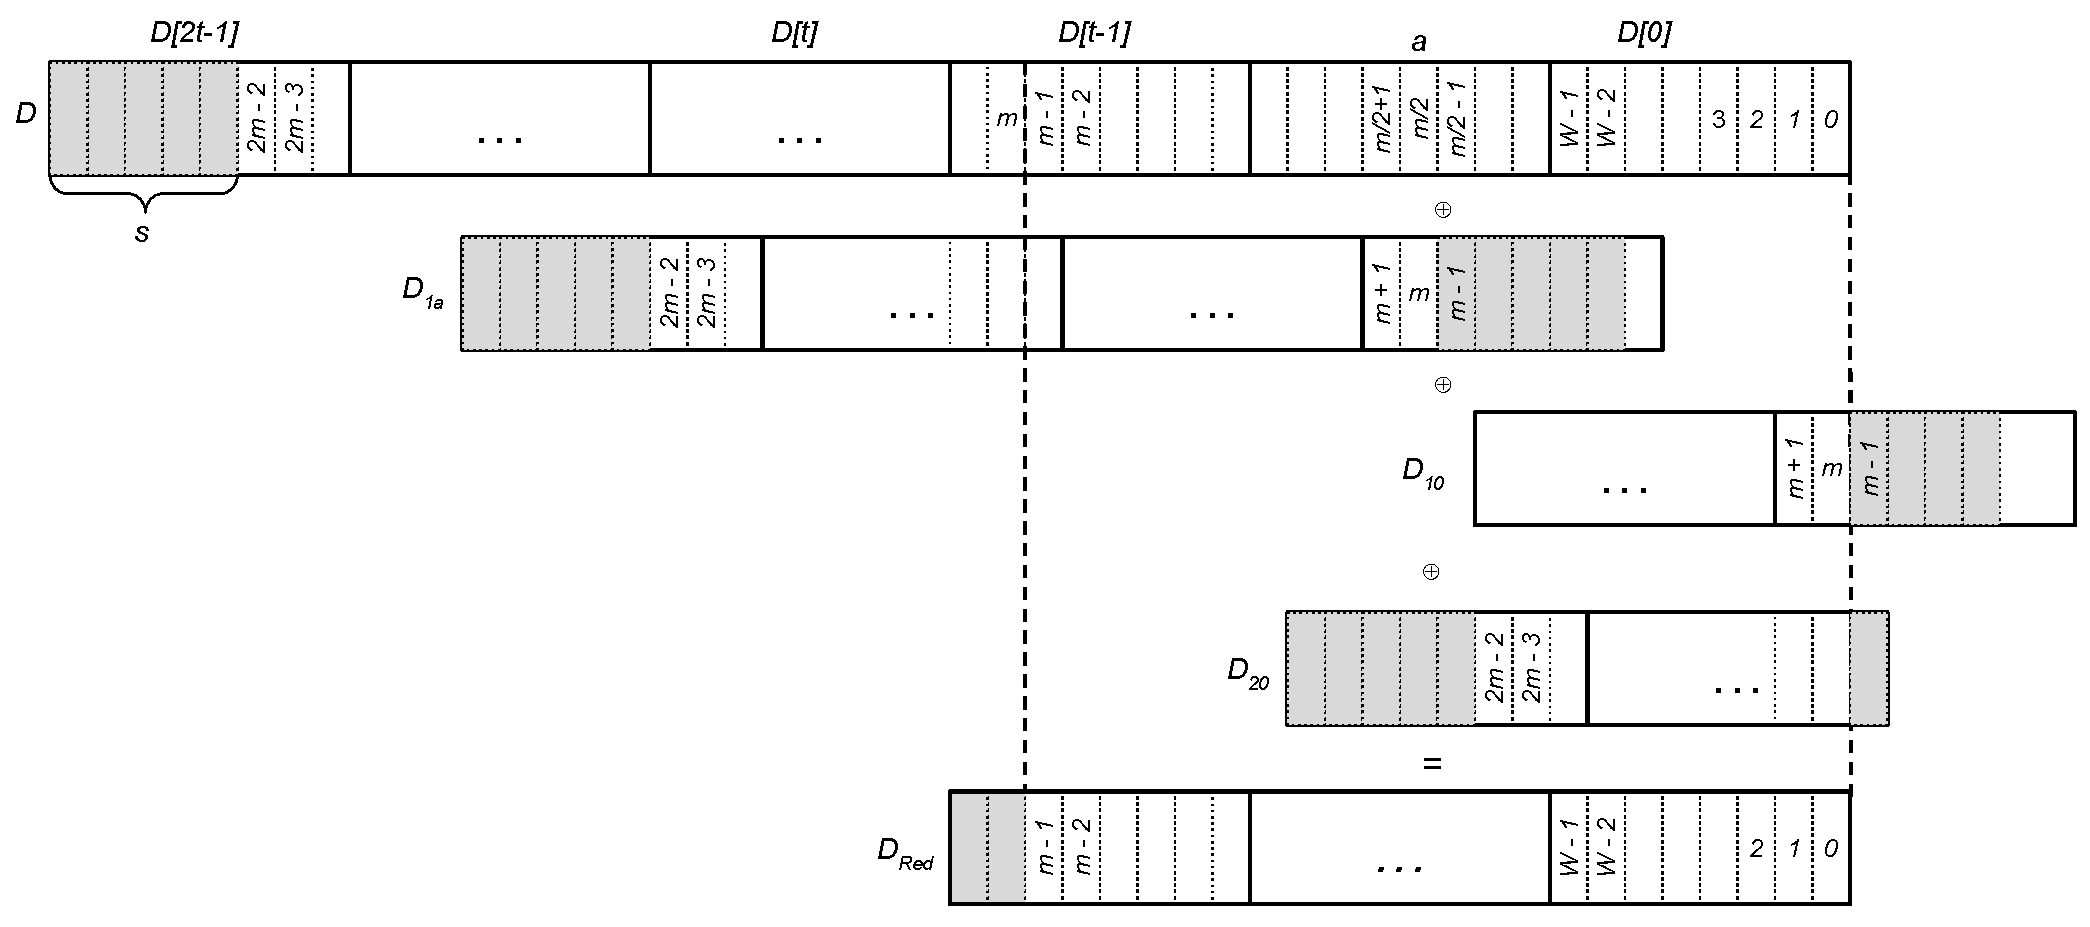
\includegraphics[width = \columnwidth]{figures/reduction-equally-spaced.pdf}
\caption{Word operation of the Algorithm \ref{alg:equallyspaced:word:operation} where $D[2t-1]$ is used.}
\label{fig:word:operation:alg:a1:low2}
\end{figure}

\begin{algorithm}
  \begin{algorithmic}[1]
  \REQUIRE $D[2t-2,0]$,$t$, $m$, $W$
  \ENSURE $D_{Red = D[t-1,0]}$
  \STATE $u \gets tW - m$
  \STATE $h \gets W - u$
  \STATE $T \gets D[t-1] \ShiftRight h$
  \STATE $D[0] \gets D[0] \oplus T \oplus (D[t] \ShiftLeft u) \oplus (T \ShiftLeft 1) \oplus (D[t] \ShiftLeft (u+1)$ \label{alg:a1:low:primeira-linha}
  \FOR{$i \gets 1$ \textbf{to} $t-3$}
    \STATE $D[i] \gets D[i] \oplus (D[i+t-1] \ShiftRight h) \oplus (D[i+t-1] \ShiftRight (h-1)) \oplus (D[i+t] \ShiftLeft u) \oplus (D[i+t] \ShiftLeft (u+1))$
    \ENDFOR
  \STATE $T \gets D[2t-2] \ShiftLeft (2u+1-W)$\ \COMMENT{This avoid using \& to reset unused bits}
  \STATE $D[t-2] \gets D[t-2] \oplus (D[2t-3] \ShiftRight h) \oplus (D[2t-3] \ShiftRight (h-1)) \oplus (T \ShiftRight u) \oplus (T \ShiftRight (u+1))$
  \RETURN $D_{Red}$
  \caption{Reduction algorithm by word for $x^m + x + 1$, from $D[2t-2]$.}
  \label{alg:word:a1:low}
\end{algorithmic}
\end{algorithm}

We have $4$ XORs in line \ref{alg:a1:low:primeira-linha}, $4(t-3)$ XORs in line 5, and $4$ XORs in line 8. The total is $$N_\oplus = 4t-4.$$

We have $$N_{Shifts} = 4t-4.$$

\subsection{Word operation of the case $a<m/2$}\label{sec:word:operation:alg:a2}
Figure \ref{fig:word:operation:alg:a2} is a representation of the case $a<m/2$. In the figure, $D$ is the element to be reduced, $D_a$ are the bits reduced by the exponent $a$ and $D_0$ are the bits reduced by $0$. $D_{Red} = D \BitXOR D_a \BitXOR D_0$ is the reduced element. The hatched bits (shaded in figure) should be set to 0.
\begin{figure}[htb]
  \centering
  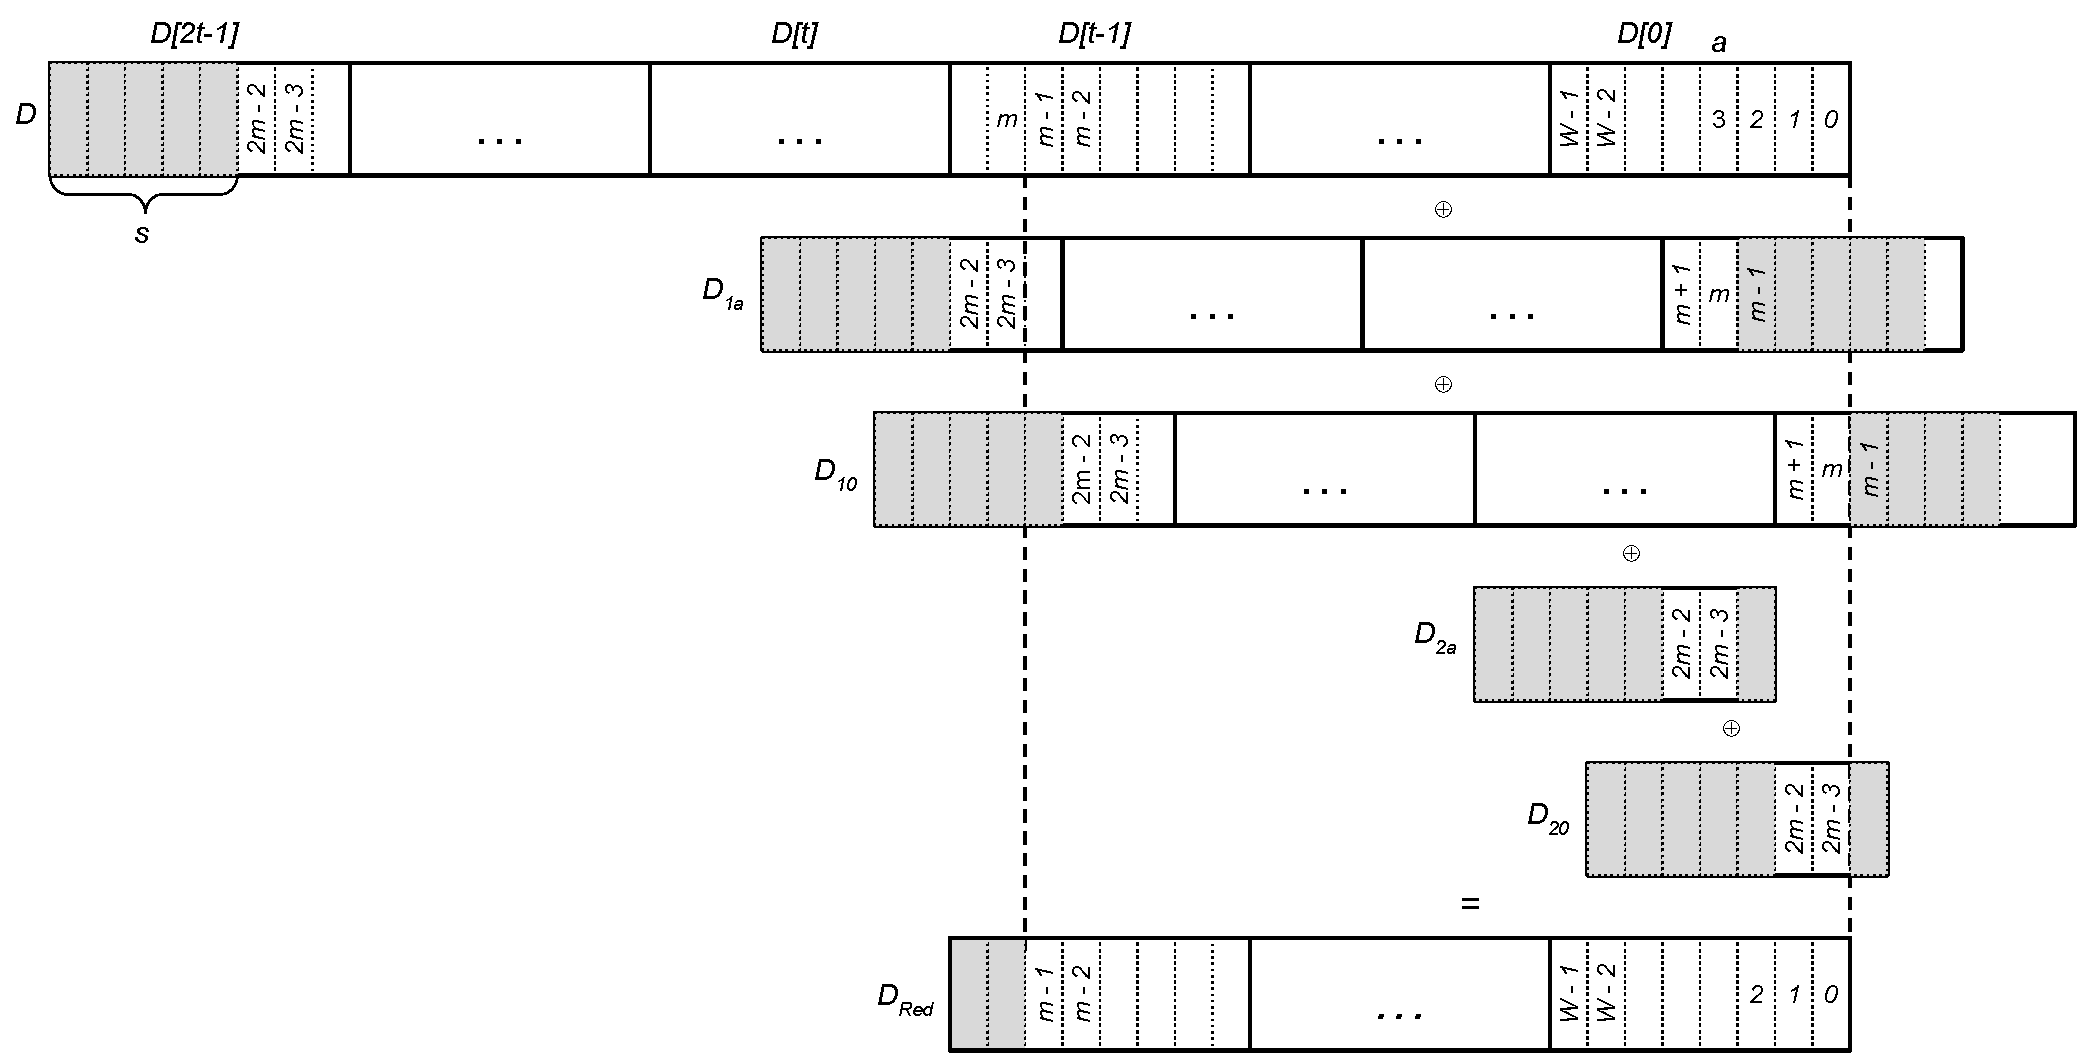
\includegraphics[width = \columnwidth]{figures/two-elements-reduction-a-6.pdf}
\caption{Word operation of the case $a<m/2$.}
\label{fig:word:operation:alg:a2}
\end{figure}
\\

\subsection{Word operation of the  Algorithm~\ref{alg:esp}}\label{sec:word:operation:alg:esp}
Figure \ref{fig:word:operation:alg:esp} is a representation of the algorithm \ref{alg:esp}. In the figure, $D$ is the element to be reduced, $D_a$ are the bits reduced by the exponent $a$ and $D_0$ are the bits reduced by $0$. $D_{Red} = D \BitXOR D_a \BitXOR D_0$ is the reduced element. The hatched bits (shaded in figure) should be set to 0.
\begin{figure}[htb]
  \centering
  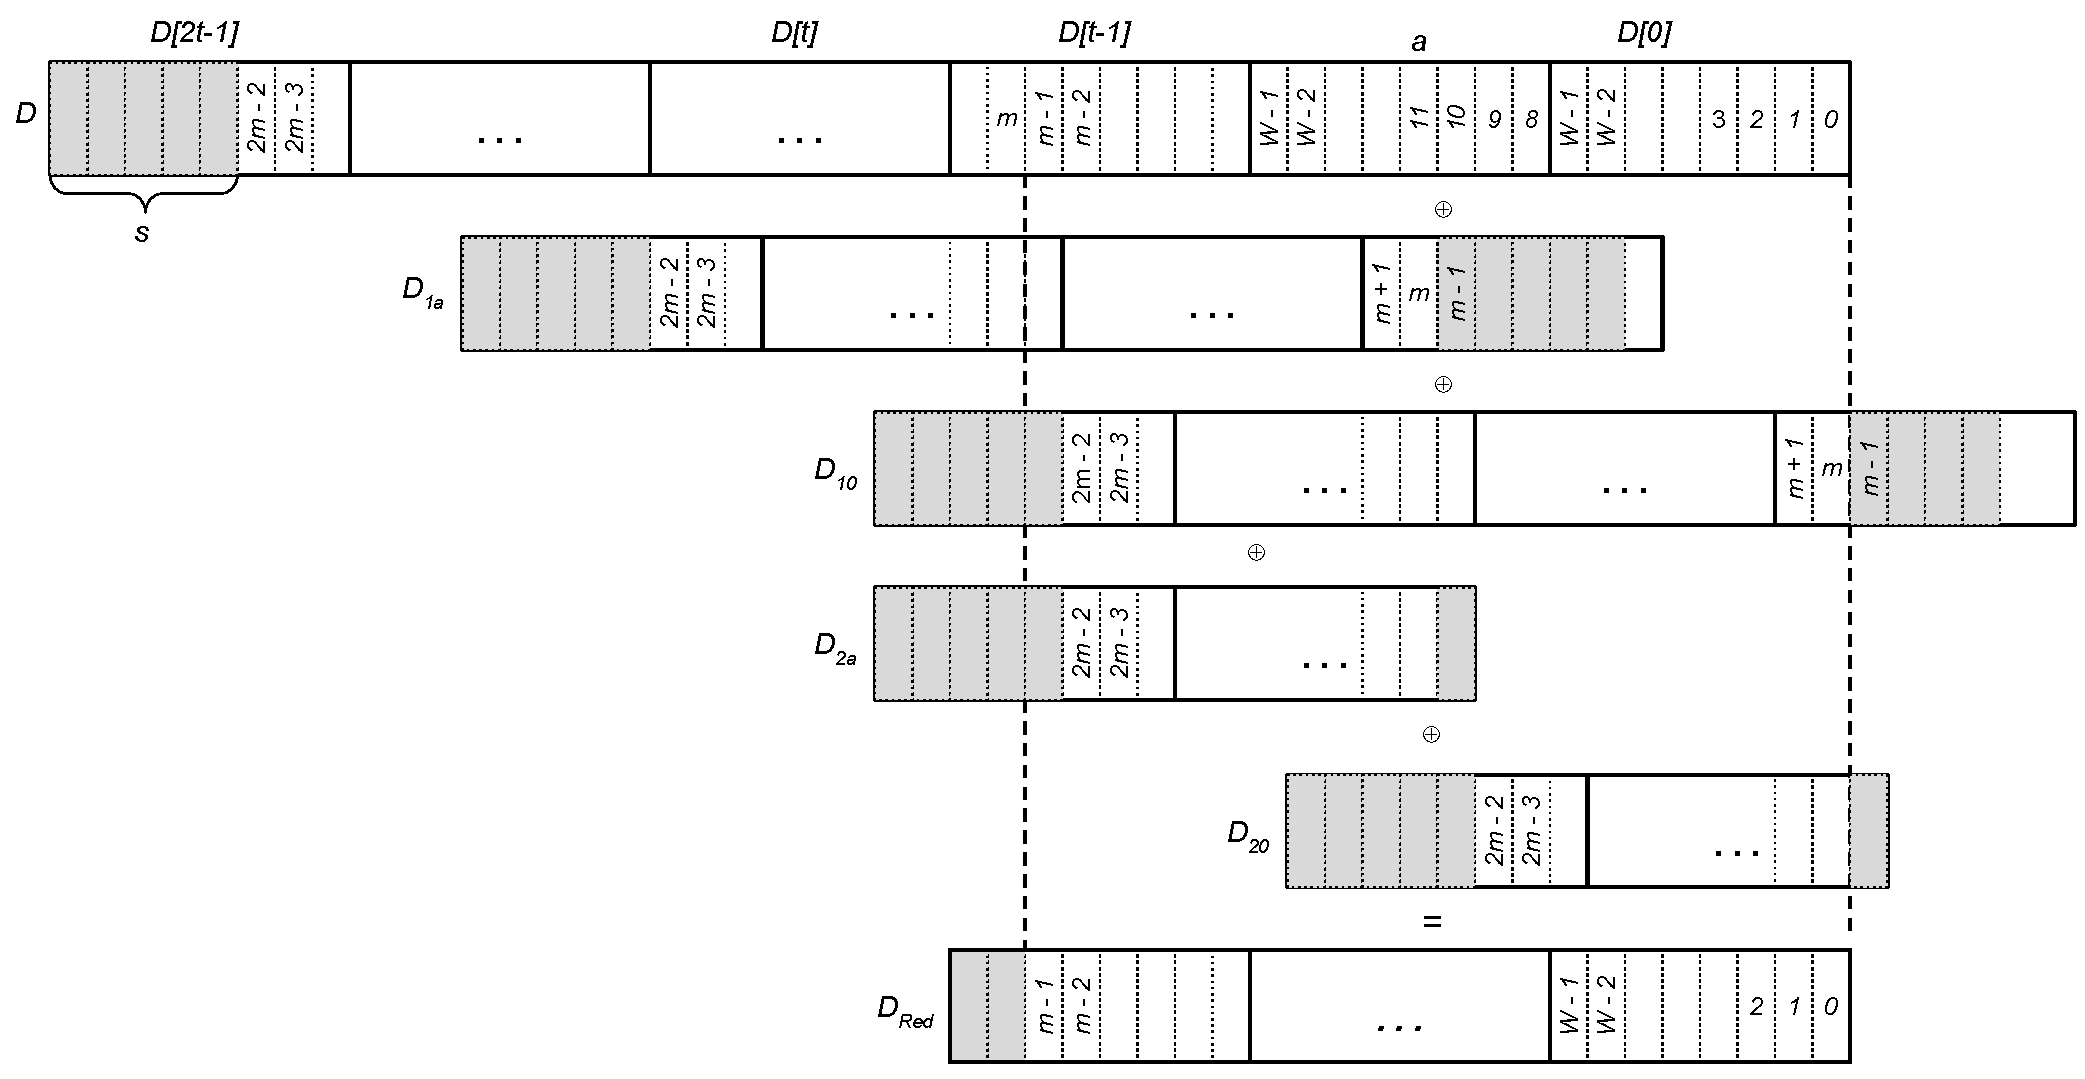
\includegraphics[width = \columnwidth]{figures/two-elements-reduction-a-11.pdf}
\caption{Word operation of the Algorithm \ref{alg:esp}.}
\label{fig:word:operation:alg:esp}
\end{figure}
\\

\subsection{Word operation of the  Algorithm~\ref{alg:general:bit:operation}}\label{sec:word:operation}

The word-oriented versions of the algorithm can be created by noticing the bit access pattern. The XOR operation pattern can be thought of XORing two ranges

Each of them perform a XOR operation between all bits in a certain range and counterparts a fixed distance away. This access pattern allows word-level parallelism. There are four issues that need to be paid attention to:

\textbf{Misaligned start:}
The loop starts at $2m -2$, which may not align with the word length ($W \nmid 2m-2$). To avoid overwriting the upper bits of this incomplete word we must clear them from the \texttt{src} word.

\textbf{Misaligned ends:}
The fix is identical to the misaligned start, where we clear the extra bits from the incoming word.

\textbf{Misaligned source:}
The source/incoming word may not be aligned to word boundaries either. In this case we need to pull bits from the next word too, shifting both of them for correct placement. Unfortunately this issue affects the start and ends word too, further complicating their treatment.

\textbf{Too small distances:}
Finally, if the distance between the XOR'ed words ($m-a$, $m$, respectively) is smaller than $W/2$, the same bit will be written and read in the same word-step. This is not possisble with a single operation, and requires handling each word in mulitple parts. This is suboptimal and should be avoided by better choices of $m$, $a$ and $W$.

Other bit-level operations are emulated with word masks and shifts.

To help transforming an algorithm in its word-parallel version we introduce the following helper functions. Notice the function calls can be inlined and all conditionals are open for static analysis (the final algorithm should contain no conditionals if optimized properly).

\begin{algorithm}
\begin{algorithmic}[1]
  \REQUIRE $dst$, $src$, $W$, $C[]$
  \STATE $mask \gets 1 << (src \mod W)$
  \STATE $C[dst / W] \gets C[dst / W] \oplus (C[src / W] \land mask) << (dst \mod W - src \mod W)$
  \caption{\texttt{XOR\_BIT}: Single bit XOR inside word}
\end{algorithmic}
\end{algorithm}

\begin{algorithm}
\begin{algorithmic}[1]
  \REQUIRE $dst$, $src$, $W$, $C[]$
  \STATE $left \gets C[src / W] >> (src \mod W)$
  \STATE $right \gets C[src / W + 1] << (W - src \mod W)$
  \STATE $C[dst / W] \gets C[dst / W] \oplus (left \lor right)$
  \caption{\texttt{XOR\_WORD}: Whole word XOR with possibly misaligned source}
\end{algorithmic}
\end{algorithm}

\begin{algorithm}
\begin{algorithmic}[1]
  \REQUIRE $dst$, $src$, $n\_bits$, $W$, $C[]$
  \STATE $shift \gets src \mod W$
  \STATE $left\_n\_bits \gets \min(n\_bits, W - shift)$
  \STATE $leftmask \gets ((1 << left\_n\_bits) - 1) << shift$
  \STATE $left \gets (C[src / W] \land leftmask) >> shift$
  \STATE $right\_n\_bits \gets n\_bits - left\_n\_bits$
  \IF{$right\_n\_bits > 0$}
    \STATE $rightmask \gets (1 << right\_n\_bits) - 1$
    \STATE $right \gets (C[src/W+1] \land rightmask) << left\_n\_bits$
  \ELSE
    \STATE $right \gets 0$
  \ENDIF
  \STATE $C[dst/W] = C[dst/W] \oplus ((left | right) << (dst \ W))$
  \caption{\texttt{XOR\_PARTIAL\_WORD}: XOR a range of bits inside a word, with possibly misaligned source}
\end{algorithmic}
\end{algorithm}

\begin{algorithm}
\begin{algorithmic}[1]
  \REQUIRE $start\_dst$, $end\_dst$, $distance$, $W$, $C[]$
  \IF{$end\_dst/W = start\_dst/W$}
    \STATE \texttt{XOR\_PARTIAL\_WORD}($start\_dst$, $start\_dst + distance$, $end\_dst - start\_dst$, $W$, $C$)
  \ELSE
    \IF{$start\_dst \ W \neq 0$}
      \STATE $remaining = W - (start\_dst \ W)$
      \STATE \texttt{XOR\_PARTIAL\_WORD}($start\_dst$, $start\_dst + distance$, $remaining$, $W$, $C$)
      \STATE $start\_dst \gets start\_dst + remaining$
    \ENDIF
    
    \STATE $rounded\_end \gets (end\_dst / W) * W$
    \STATE $dst \gets start\_dst$
    \WHILE{$dst < rounded\_end$}
      \STATE \texttt{XOR\_WORD}($dst$, $dst + distance$, $W$, $C$)
      \STATE $dst \gets dst + W$
    \ENDWHILE
    
    \IF{$end\_dst \ W \neq 0$}
      \STATE \texttt{XOR\_PARTIAL\_WORD}($rounded\_end$, $rounded\_end + distance$, $end\_dst \ W$, $W$, $C$)
    \ENDIF
  \ENDIF
  \caption{\texttt{XOR\_RANGE}: XOR a range of bits (across many words) with an equivalent range a certain distance away}
\end{algorithmic}
\end{algorithm}


And the word-transformed algorithms are:

\begin{algorithm}
\begin{algorithmic}[1]
  \REQUIRE $m$, $a$, $W$, $C\left[0,\ceil*{\frac{2m-2}{W}}\right]$
  \ENSURE $C[0,m-1]$
  \STATE \texttt{XOR\_RANGE}($a$, $a+m$, $m$, $W$, $C$)
  \STATE \texttt{XOR\_RANGE}($0$, $a-1$, $m$, $W$, $C$)
  \RETURN $C$
  \caption{Simple word-parallel reduction algorithm for $x^m + x^a +1$, $a = \frac{m}{2}$}
  \label{alg:equallyspaced:word:operation}
\end{algorithmic}
\end{algorithm}

\begin{algorithm}
\begin{algorithmic}[1]
  \REQUIRE $m$, $a$, $W$, $C\left[0,\ceil*{\frac{2m-2}{W}}\right]$
  \ENSURE $C[0,m-1]$
  \STATE $start\_src \gets m$
  \STATE $step\_size \gets m - a$
  \WHILE{$start\_src \le 2m - 2$}
    \STATE \texttt{XOR\_RANGE}($a$, $a + 2m-2 - start\_src$, $start\_src - a$, $W$, $C$)
    \STATE $start\_src \gets start\_src + step\_size$
    \STATE $step\_size \gets 2 \times step\_size$
  \ENDWHILE
  \STATE \texttt{XOR\_RANGE}($0$, $m$, $m$, $W$, $C$)
  \RETURN $C$
  \caption{Alternative reduction algorithm, uses more XORs but less calls to \texttt{XOR\_RANGE}, may be useful for certain architectures.}
  \label{alg:new:word:operation}
\end{algorithmic}
\end{algorithm}

\section{Example Algorithms}

The algorithm \ref{alg:new:word:operation} proposed can be applied to specific trinomials with fixed parameters. For example, for the commonly used field $x^{233} + x^{74} + 1$, with 32-bit words, this results in algorithm \ref{alg:233-32:word:operation}. The total number of operations of this algorithm is 19 XORs, 16 ORs, 5 ANDs and 35 shifts, for a total of 75 word operations.

\begin{algorithm}
\begin{algorithmic}[1]
  \REQUIRE $C\left[0,\ceil*{\frac{2m-2}{W}}\right]$
  \ENSURE $C[0,m-1]$
  \STATE $C[2] \gets C[2] \oplus ((C[7] \land \texttt{0x7ffffe00}) << 1)$
  \STATE $C[3] \gets C[3] \oplus ((C[7] >> 31) \lor (C[8] << 1))$
  \STATE $C[4] \gets C[4] \oplus ((C[8] >> 31) \lor (C[9] << 1))$
  \STATE $C[5] \gets C[5] \oplus ((C[9] >> 31) \lor (C[10] << 1))$
  \STATE $C[6] \gets C[6] \oplus ((C[10] >> 31) \lor (C[11] << 1))$
  \STATE $C[7] \gets C[7] \oplus ((C[11] >> 31) \lor (C[12] << 1))$
  \STATE $C[8] \gets C[8] \oplus ((C[12] >> 31) \lor (C[13] << 1))$
  \STATE $C[9] \gets C[9] \oplus ((C[13] >> 31) \lor ((C[14] \land \texttt{0x1ffff}) >> 1))$
  \STATE $C[2] \gets C[2] \oplus ((C[12] \land \texttt{0x3fffff00}) << 2)$
  \STATE $C[3] \gets C[3] \oplus ((C[12] >> 30) \lor (C[13] << 2))$
  \STATE $C[4] \gets C[4] \oplus ((C[13] >> 30) \lor ((C[14] \land \texttt{0x1ffff}) >> 2))$
  \STATE $C[0] \gets C[0] \oplus ((C[7] >> 9) \lor (C[8] << 23))$
  \STATE $C[1] \gets C[1] \oplus ((C[8] >> 9) \lor (C[9] << 23))$
  \STATE $C[2] \gets C[2] \oplus ((C[9] >> 9) \lor (C[10] << 23))$
  \STATE $C[3] \gets C[3] \oplus ((C[10] >> 9) \lor (C[11] << 23))$
  \STATE $C[4] \gets C[4] \oplus ((C[11] >> 9) \lor (C[12] << 23))$
  \STATE $C[5] \gets C[5] \oplus ((C[12] >> 9) \lor (C[13] << 23))$
  \STATE $C[6] \gets C[6] \oplus ((C[13] >> 9) \lor (C[14] << 23))$
  \STATE $C[7] \gets C[7] \oplus ((C[14] \land \texttt{0x3fe00}) >> 9)$
  \RETURN $C$
  \caption{Reduction algorithm for $x^{233} + x^{74} + 1$ with 32-bit words}
  \label{alg:233-32:word:operation}
\end{algorithmic}
\end{algorithm}


% http://download.springer.com/static/pdf/429/chp253A10.1007252F978-3-642-33481-8_10.pdf?originUrl=http3A2F2Flink.springer.com2Fchapter2F10.10072F978-3-642-33481-8_10&token2=exp=1441741030~acl=2Fstatic2Fpdf2F4292Fchp25253A10.100725252F978-3-642-33481-8_10.pdf3ForiginUrl3Dhttp253A252F252Flink.springer.com252Fchapter252F10.1007252F978-3-642-33481-8_10*~hmac=7fed14b6b9363e3a95601342a355c7f5b9a630f6dcad462d10adb7e8ff1552b9
%http://ieeexplore.ieee.org/xpls/abs_all.jsp?arnumber=6927388&tag=1
%http://www.sciencedirect.com/science/article/pii/S107157971400121X
%https://eprint.iacr.org/2007/192.pdf


\section{NIST Polynomials and their costs}

NIST Binary Polynomials and their costs (Guide to Elliptic Curve Crytography - Hankerson - page 76

\begin{itemize}
\item $x^{163} + x^7 + x^6 + x^3 + 1$ - $C[0..10]$, 41 XORs, 36 SHIFTs, 1 AND = 78 operations
\item $x^{233} + x^{74} + 1$ - $C[0..15!]$, 35 XORs, 35 SHIFTs, 1 AND = 71 operations
\item $x^{283} + x^{12} + x^7 + x^5 + 1$ - $C[0..17]$, 76 XORs, 76 SHIFTs, 1 AND = 153 operations
\item $x^{409} + x^{87} + 1$ - $C[0..25]$, 54 XORs, 54 SHIFTs, 1 AND = 109 operations
\item $x^{571} + x^{10} + x^5 + x^2 + 1$ - $C[0..35]$, 148 XORs, 148 SHIFTs, 1 AND = 297 operations
\end{itemize}


Pentanomials of same degree from the family $x^{b+2c} + x^{b+c} + x^b + x^c + 1$

\begin{itemize}
\item $x^{233} + x^{158} + x^{83} + x^{74} + 1$, score 3.717, $k_a=4$
\item $x^{163} + x^{117} + x^{71} + x^{46} + 1$, score 3.982, $k_a=4$
\item $x^{409} + x^{294} + x^{179} + x^{115} + 1$, score 4.015, $k_a=4$
\item $x^{409} + x^{337} + x^{265} + x^{72} + 1$, score 4.457, $k_a=6$
\item $x^{233} + x^{217} + x^{201} + x^{16} + 1$, score 7.240, $k_a=15$
\item ??571??
\end{itemize}